
\section{Association Analysis}

\begin{breakbox}
\boxtitle{FP Growth:}
\begin{center}
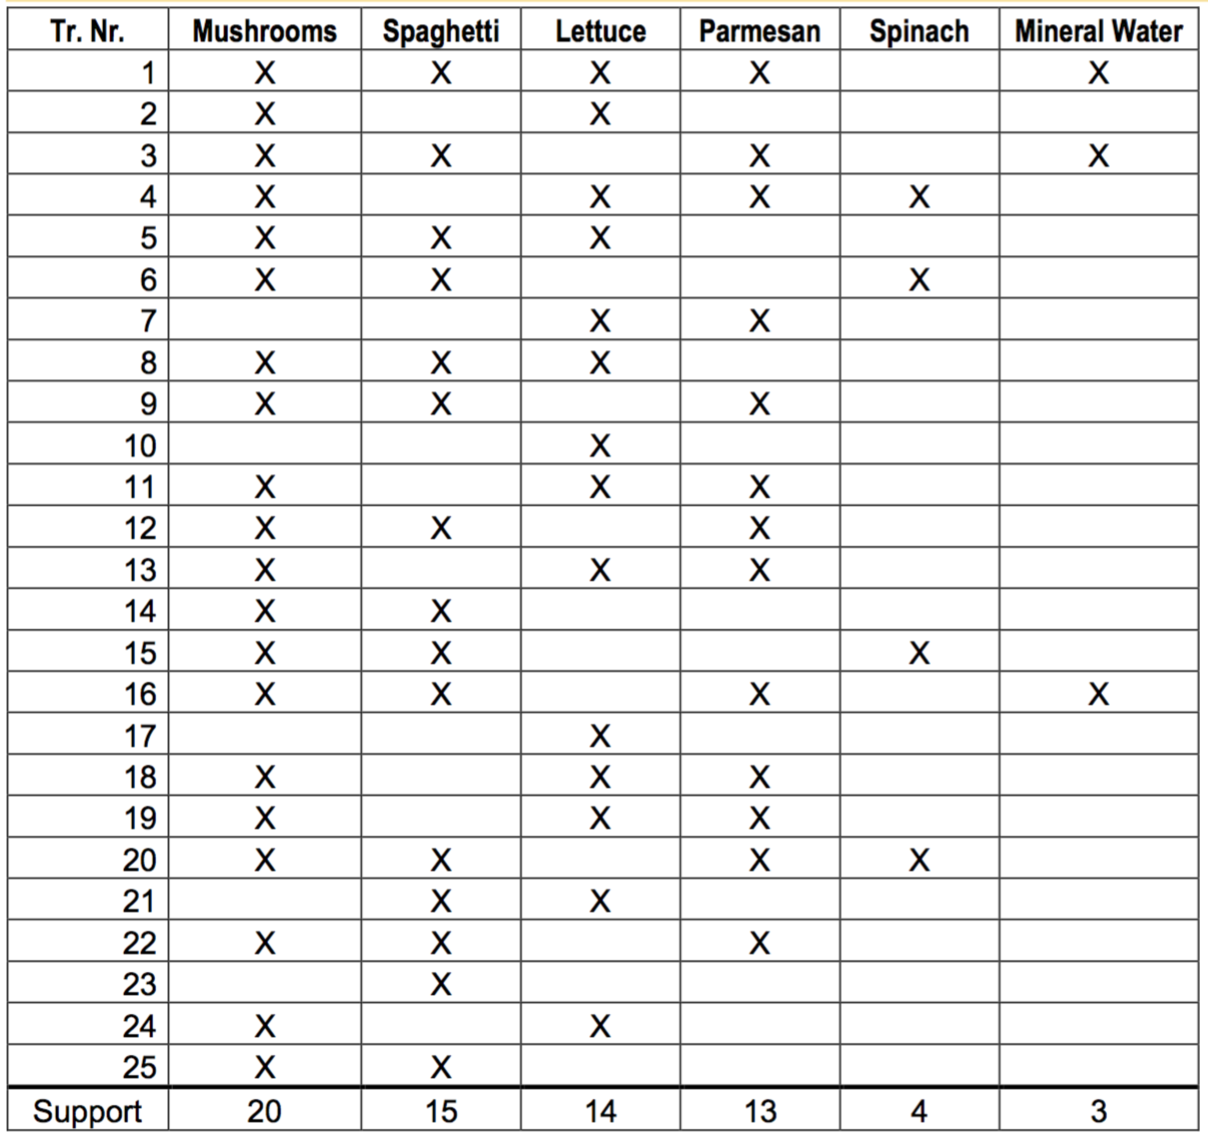
\includegraphics[width=.15\textwidth]{slides_images/fp_growth_data}
\end{center}
Algorithm:
\begin{itemize}
	\item Step 1: full table scan and determination of support count for 1-item-sets.
	\item Step 2:
		\begin{itemize}
			\item select items with at least minimum support.
			\item sort items by support count in descending order / corresponds to a reordering of columns (projection).
			\item table is processed in that order.
		\end{itemize}
	\item Step 3: Generating an FP-tree:
		\begin{itemize}
			\item create empty root node.
			\item for each transaction in reordered table:
				\begin{itemize}
					\item add a new branch to the tree.
					\item nodes of this branch correspond to the sequence of attributes in the reordered table.
					\item existing parts of branches (prefixes) will not be created but a counter on each node in the prefix is incremented by 1.
				\end{itemize}
			\item for quick tree traversals
				\begin{itemize}
					\item additional item header table: For each item it holds pointers to every node containing that item.
				\end{itemize}
		\end{itemize}
	\item Step 4: Mining the FP-tree:
		\begin{itemize}
			\item Start with the least frequent item (last column in the reordered table).
			\item For each frequent item.
				\begin{itemize}
					\item generate its conditional pattern base, i.e. a list of all existing paths in the tree leading to that item (all prefixes).
					\item generate its conditional FP-tree, i.e. all frequent enough ($\geq$ minimum support) paths leading to the item in the conditional pattern base (frequent prefixes).
					\item combine each frequent prefix with the item itself (the suffix), forming a frequent pattern.
				\end{itemize}
			\item continue with next item in reversed table order.
		\end{itemize}
\end{itemize}
Exercise: Identify frequent itemsets with minimum support = 0.2, employing the FP-growth method.
\begin{center}
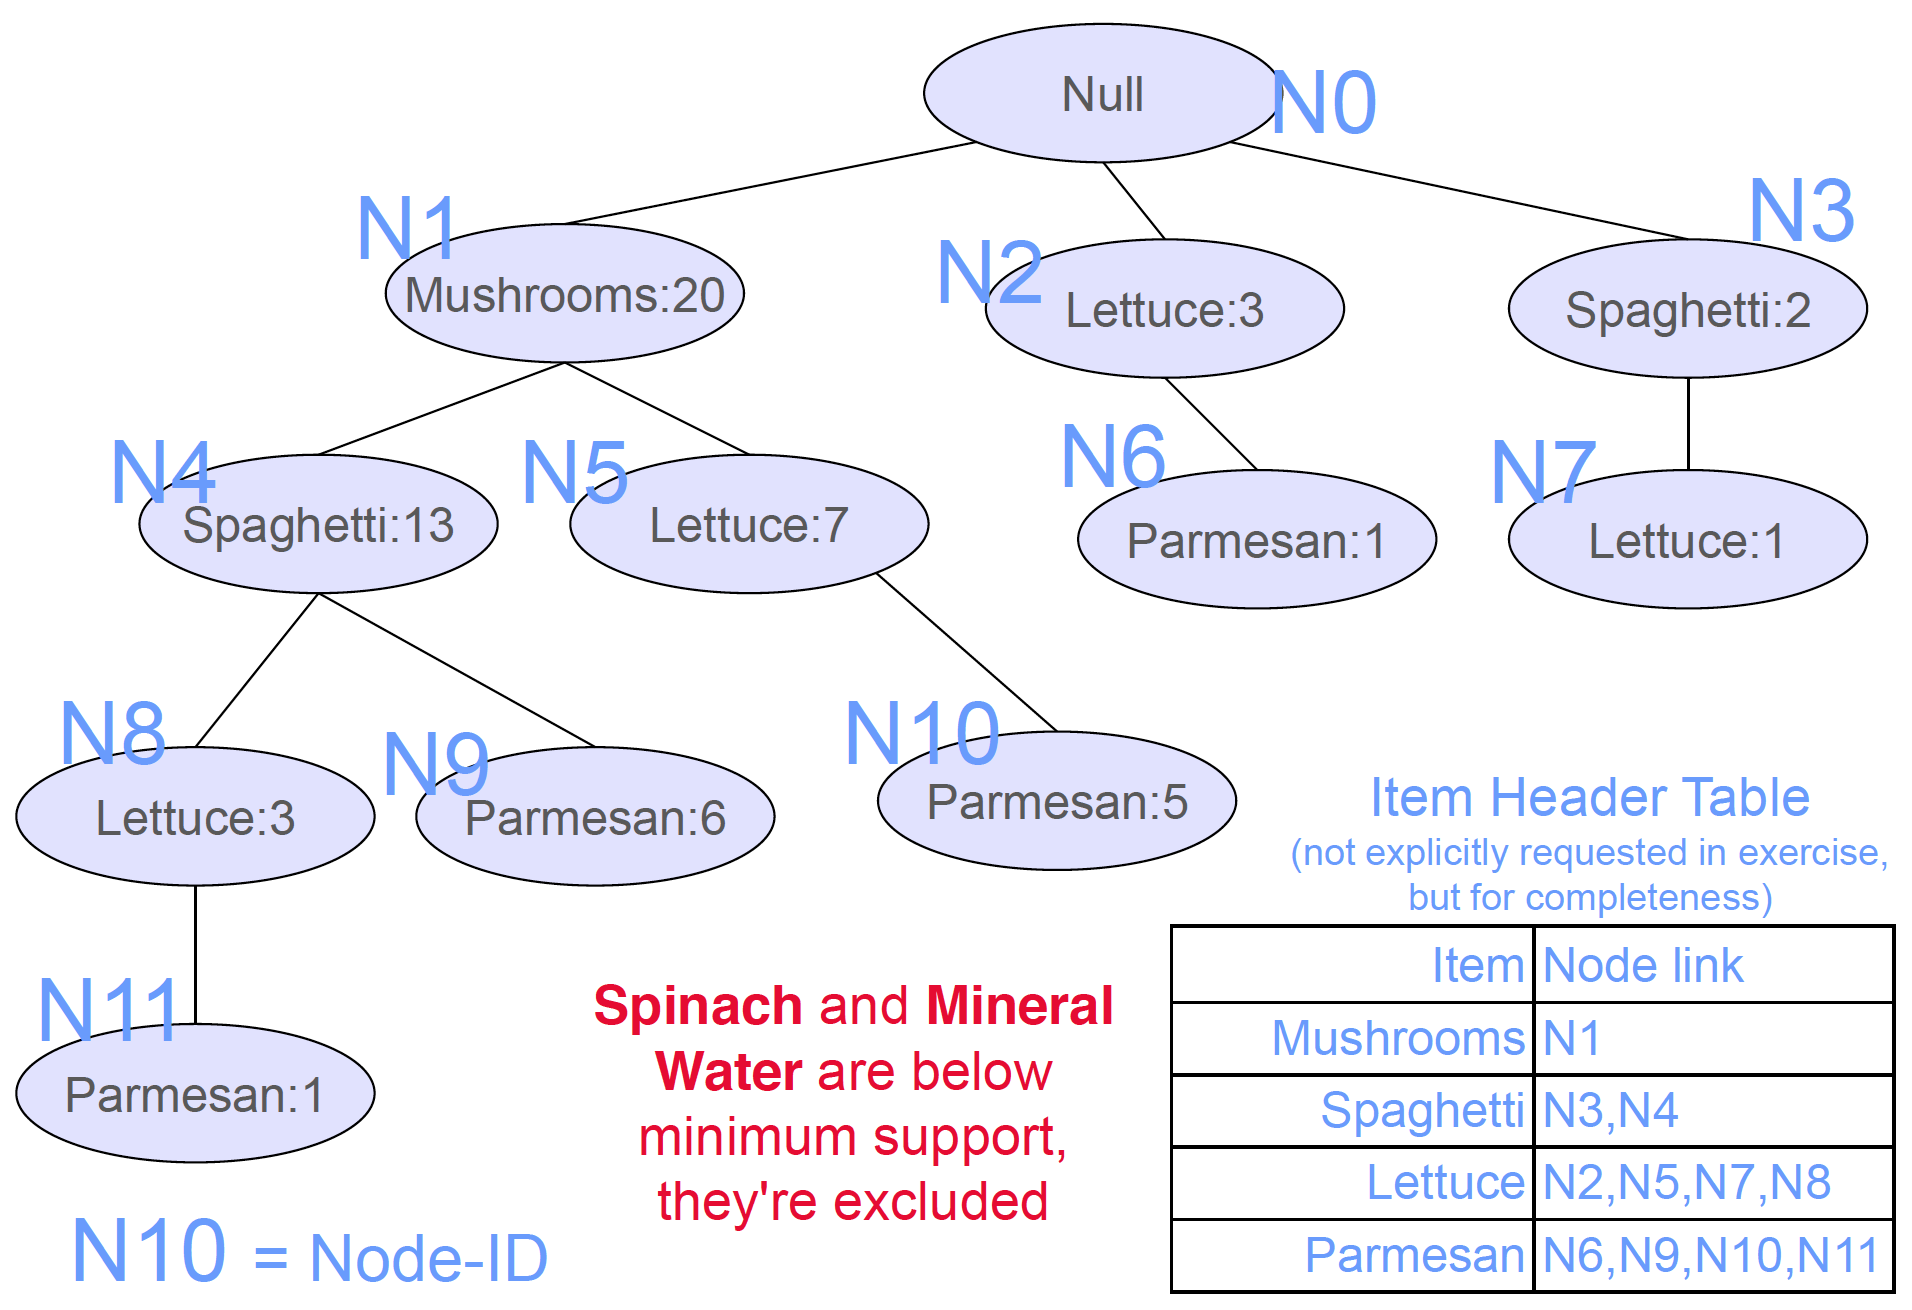
\includegraphics[width=.15\textwidth]{slides_images/fp_tree}
\end{center}
This results in the following table:
\begin{center}
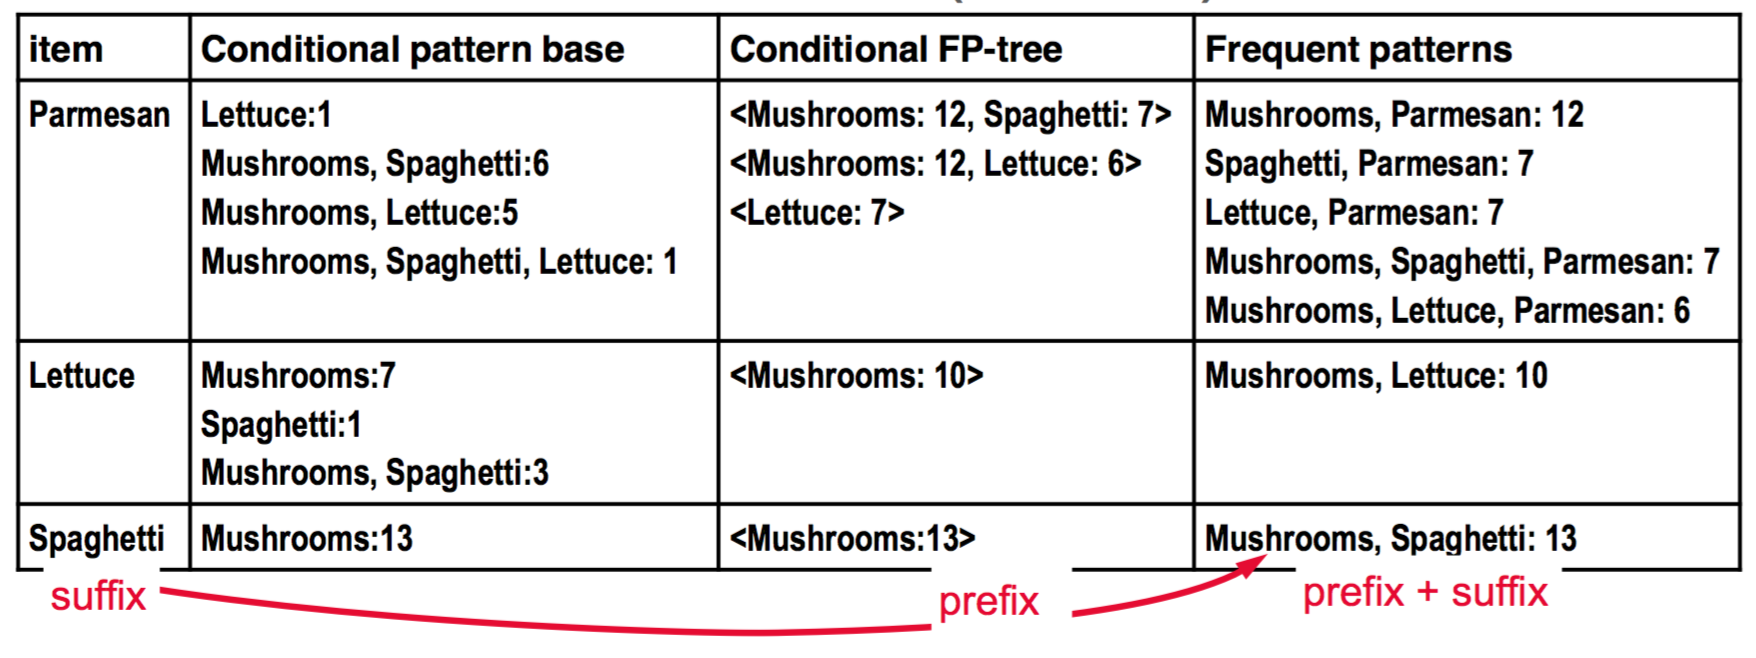
\includegraphics[width=.15\textwidth]{slides_images/frequent_patterns}
\end{center}
\end{breakbox}

